\documentclass{article}
\usepackage[utf8]{inputenc}
\usepackage[maxcitenames=1,style=numeric]{biblatex}
\usepackage{amsmath}
\usepackage{amssymb}
\usepackage{amsthm}
\usepackage{tcolorbox}
\usepackage{graphicx}
\usepackage{algorithm}
\usepackage{algorithmic}
\usepackage{subfig}
\usepackage{hyperref}
\usepackage{cleveref}
\usepackage{thmtools}
\usepackage{thm-restate}
\usepackage{enumerate}
\usepackage{xcolor}

\topmargin -.5in
\textheight 9in
\oddsidemargin -.25in
\evensidemargin -.25in
\textwidth 7in

\title{Machine Learning based TIR predictor}
\author{}
\date{\today{}}

\bibliography{ref.bib}
\DeclareUnicodeCharacter{2212}{-}
\begin{document}

\maketitle

\section{Introduction}

One of the main tenets of synthetic biology is design, evaluation and standardisation of genetic parts \cite{Brophy2014,Canton2008,Stanton2014}. This can be done in variety of ways, most of each involve designing the DNA sequence in CAD software and then physically testing it in a laboratory. Alternative to this is computer modelling and prediction of part behaviour based on the designed DNA sequence or design of DNA sequence based on expected function \cite{Yeoh2019,Nielsen2016}. Most of these models are based on either the thermodynamic properties of the involved molecules (DNA, RNA, proteins among others) or empirically obtained values describing a relevant to design value, like Translation Initiation Rate (TRI) in case of Ribosome Binding Sites (RBS) \cite{Xia1998,Chen2013,Reeve2014}.\\
According to Reeve \emph{et al.} there are three main RBS calculators, all predicting the TRI based on the thermodynamic properties of the RBS and the ribosome \cite{Seo2013,Na2010,Salis2009}. Predictions from all of these models are relatively good ($R^2 >0.8$), there come with a number of caveats: i) they rely on calculations of free energies that can be hard to calculate ii) in general, the models' accuracy is improved by increasing the number of phenomenons taking place during the translation, but this can lead to paradoxically decreased model accuracy due to accumulation of errors \cite{EspahBorujeni2016} and iii) by using deterministic coefficients to calculate energies one disregards often stochastic nature of processes in the cells which again increases perceived prediction error \cite{Goss1998}. \\
Synthetic biology is currently going through a phase of exponential increase in volume of data produced during experiments. \cite{Freemont2019} New experimental methods heavily relying on advances in automation and microfludics allow unprecedented precision and throughput in data generation. These new data-sets can be combined with data reliant machine learning algorithms to generate new models and predictors for use in synthetic biology \cite{Camacho2018}. In the past few years there was a significant uptick of Machine Learning based approaches to synthetic biology. Jervis \emph{et al.} used support vector machine and neural network to optimise production of monoterpenoid in \emph{Esherichia coli} \cite{Jervis2019}. Similarly, Costello \emph{et al.} have used a number of machine learning approaches to analyse time-series multiomics data to predict metabolic pathway bahaviour \cite{Costello2018}. There were also successful attempts at using deep learning techniques for analysis of big data-sets \cite{Alipanahi2015,Angermueller2016}. However, the use of machine learning in synthetic biology is still in its infancy and will require additional research to show its full potential. \\
Here we present a machine learning workflow for building a RBS translation rate predictor based on fluorescence data from cultures. RBS being one of the key genetic elements controlling protein expression and at he same time having a relatively short sequence is a perfect target for establishing workflows that can be later translated to more complicated systems. We have used Gaussian Process-Upper Confidence Bound and Bandits algorithms to analyse and optimise the initiation rates of the designed RBS.

\section{Genetic device design}
There is a number of qualities that impact the translation rate, but chief among them are concerned with how the ribosome recognises and binds to the RBS sequence \cite{Chen1994,Vellanoweth1992}. In \emph{E. coli} the RBS is usually located in the 20 bases downstream of the start codon. The RBS usually has a distinguishable, consensus, core sequence called the Shine-Dalgarno sequence, which in \emph{E. coli} is AGGAGG. Here, we put that 20 bp long sequence into focus with main emphasis being put on the 6bp core region (Figure 1).\\
The RBS controls expression of the Green Fluorescent Protein (GFP) in its mut3b variant. By controlling expression of a fluorescent protein with the RBS we can quickly assess the perceived TIR by measuring fluorescence of cells harbouring the device. Finally, the mRNA is transcribed from an IPTG-inducible promoter pLlacO-1. By making the whole device inducible we can synchronise the start of the expression of the GFP in all the cultures by inducing them at the same optical density (OD\textsubscript{600}) with addition of IPTG.\\


\begin{figure}[t]
    \centering
    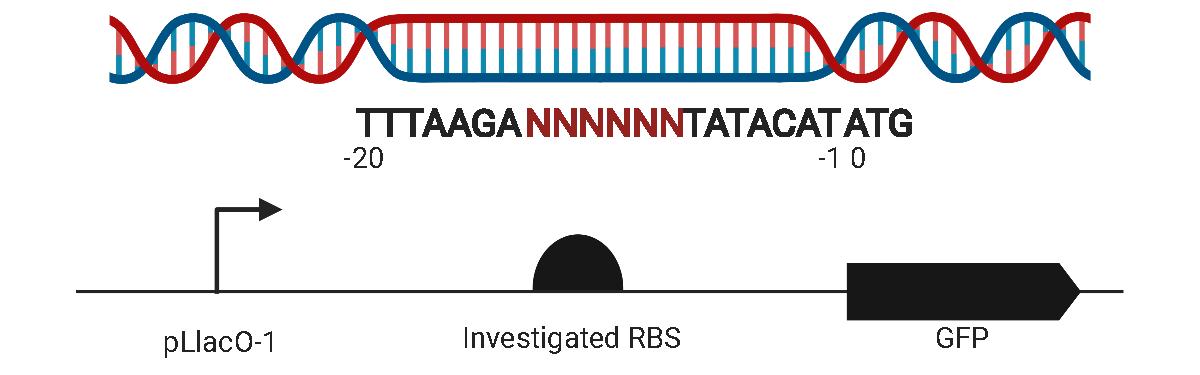
\includegraphics[scale=0.6]{plots/RBS_anatomy.pdf}
    \caption{\textbf{Diagram of the investigated sequence.} The sequence of the investigated RBS is shown with the randomised core sequence in red. The start codon of the GFP coding sequence is also shown with numbers showing relative nucleotide positions. At the bottom a simplified SBOL diagram of the genetic device is shown.}
    \label{fig: Anatomy of the randomized sequence.}
\end{figure}

\section{Method}
This will be about the DNA assembly.\\
\subsection{SynBio methods}
This will be very specifically talking about the plasmid.

\subsection{Algorithms}

\subsubsection{ Position probability matrix based sampling}


\subsubsection{Machine learning experimental design}

To automatically design the RBS sequences in batch using machine learning, we need to consider two parts: 
1) Design an regression algorithm which takes the RBS sequences as input and returns the predicted TIR scores and the confidence interval for the prediction. 
2) Design an online learning approach which recommends the RBS sequences based on the predicted TIR scores and confidence interval. 
Such online learning approach provides the $\textit{exploitation-exploration balance}$. 
We show the corresponding methods we use in the below. 

We consider our experimental design problem as the problem of sequentially optimising an unknown reward function $f: \mathcal{D} \rightarrow \mathbb{R}$, where $\mathcal{D}$ is the set containing all RBS sequence point, and $f(\mathbf{x})$ is the TIR score at $\mathbf{x}$. 
In each round $t$, we choose a set of $m$ points $\mathcal{S}_t \subset \mathcal{D}$ and observe the function values of each points in the selected set $\mathcal{S}_t$, i.e. $y_i = f(\mathbf{x}_i) + \epsilon_i$, for all $i \in \mathcal{S}$, where $\epsilon_i$ is the noise (we assume the noise is under Gaussian distribution with some unknown mean and variance). 
The noise influenced by the accuracy RBS calculator and other experimental interference (e.g. \textcolor{red}{To be added}). 
Our goal is to pick RBS sequence with the largest possible TIR score after the total number of rounds $N$. 

\begin{itemize}
    \item \textit{Gaussian process regression (GPR)}.
    A Gaussian process regression model \cite{Rasmussen2004} is a Bayesian approach to regression which provide uncertainty measurements on predictions. 
    We model $f$ as a sample from a \textit{Gaussian process} $GP(\mu(\mathbf{x}), k(\mathbf{x}, \mathbf{x'}))$, which is specified by the mean function $\mu(\mathbf{x})=\mathbb{E}[f(\mathbf{x})]$ and the kernel (or covariance) function $k\left(\mathbf{x}, \mathbf{x}^{\prime}\right)=\mathbb{E}[(f(\mathbf{x})-\left.\mu(\mathbf{x}))\left(f\left(\mathbf{x}^{\prime}\right)-\mu\left(\mathbf{x}^{\prime}\right)\right)\right]$.\\
    We choose to use \textit{spectrum kernel} \cite{leslie2001spectrum} to specify the kernel function of $GP$.  
    The spectrum kernel is widely used for classifying protein sequences \cite{leslie2001spectrum, ben2008support}, which takes two sequences as inputs and outputs a scalar value which represents the similarities between the two sequences. More precisely, $k_\ell^{\text{spec}}(\textbf{x}, \textbf{x}^\prime) =\left\langle\Phi_{\ell}^{\mathrm{spec}}(\mathbf{x}), \Phi_{\ell}^{\mathrm{spec}}\left(\mathbf{x}^{\prime}\right)\right\rangle$, where $\mathbf{x}, \mathbf{x}^\prime$ are two RBS sequences in $\mathcal{D}$ over an alphabet $\Sigma$. Denote the number of letters in the alphabet as $|\Sigma|$. $\Phi_{\ell}^{\mathrm{spec}}(\mathbf{x})$ maps the sequence $\textbf{x}$ into a $|\Sigma|^\ell$ dimensional feature space, where each dimension is the count of the number of one of the $|\Sigma|^\ell$ possible strings $s$ of length $\ell$.
    %Since the sequences in provided data have the pattern that the core area is different from each other, and other areas are similar. So the kernel for Gaussian Process we are using is the sum of kernels, for core areas we use spectrum kernel with string as input directly, and for other areas we use one-hot encoding and dot product kernel for simplicity.
    
    
    \item \textit{Upper confidence bound (UCB)}. Bandit algorithms \cite{lattimore2018bandit} provide various approaches to sequentially design an where an agent adaptively chooses one or more options among several actions based on certain policies. We consider a type of bandit algorithms, the upper confidence bound algorithm, which is based on the \textit{optimism in the face of uncertainty}. The UCB algorithm, as the name suggested, basically selects RBS sequences with the maximum upper confidence bound, i.e. $\operatorname{argmax}_{\mathbf{x}_i \in \mathcal{D}} \left( \mu_t(\mathbf{x}_i) + \beta_t \sigma_t(\mathbf{x}_i)\right)$,
    where $\beta_t$ is a hyperparmeter balancing the exploitation and exploration, 
    $\mu_t(\mathbf{x}_i), \sigma_t(\mathbf{x}_i)$ are the predicted mean and standard deviation at round $t$ for the sequence $\mathbf{x}_i$. 
\end{itemize}

Combine the two parts together, we apply \textit{Gaussian Process Upper Confidence Bound (GPUCB)} algorithm, which has been theoretically analysed by \textcite{srinivas2012information}. We show the flowchart of machine learning based experimental design in Figure \ref{fig: flowchart of machine learning based experimental design.}.


\begin{figure}[t]
    \centering
    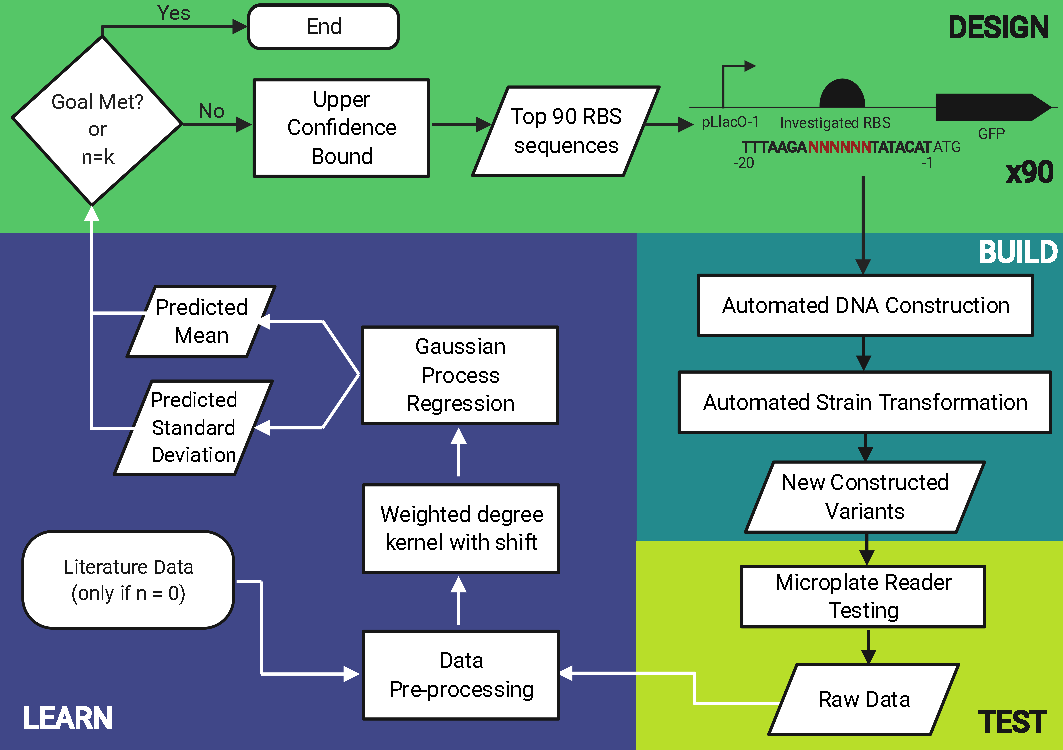
\includegraphics[scale=0.35]{plots/flowchart.pdf}
    \caption{Flowchart of machine learning based experimental design.}
    \label{fig: flowchart of machine learning based experimental design.}
\end{figure}







\section{Workflow Description}

Our experimental goal was to optimise the translation initiation rate by identifying the set of RBS sequences with top TIR scores with as fewer rounds as possible. We did this by designing a sequential experimental workflow, where we start with either randomised RBS sequences designed to explore the experimental space (round 1) or with RBS sequences recommended by the algorithm (subsequent rounds). The designs were then physically constructed in batches of 90 to fit our automated process (see \textbf{Methods} section). After constructing the plasmids harbouring the new devices are tested in microplate reader and flow cytometer. The results are then fed back to the algorithm for it to recommend the next round of designs.\\
The investigated RBS sequence is 20 bps long with the sequence TTTAAGAAGGAGATATACAT, which a known high TIR RBS that comes with the pBb series plasmids \cite{Lee2011}. In our design we focus on randomizing of the core -8 to -13 (relative to the GFP) bps of the RBS and fix others to be the same as the consensus sequence, i.e. TTTAAGA + NNNNNN + TATACAT. Since for each of the 6 position there are 4 possibilities: A, C, G, T the total feature space is $4^6$ = 4096.\\
For the first round of experiments, we design 180 (two times 90) RBS sequences based on the consensus sequence: 

\begin{enumerate}
    \item 60 RBS sequences which are subsequent single nucleotide changes of all 20 nucleotides of the original, consensus sequence. This batch is designed to show us influence of such single nucleotide changes on the overall performance of the RBS and the potential impact of changes made beyond the core part.
    \item 30 RBS sequences fully and uniformly randomised (equal probability of choosing either nucleotide for each position) 
    \item 30 RBS sequences randomised based on the position probability matrix (PPM) \textcolor{red}{we need a citation and better explanation for this}  
    \item 60 RBS sequences recommended by initial machine learning approach. For this, and subsequent design rounds, we use bandit optimisation algorithm called Gaussian Process Upper Confidence Bound (GPUCB) (see \textbf{Methods} section) \cite{srinivas2012information}. Since we don't have access to any prior data fitting our design we approximated the recommendations based on the data from \textcite{jervis2018machine}. 
\end{enumerate}{}

\begin{figure}[t]
    \centering
    \includegraphics[scale=0.7]{plots/TIR_histogram.pdf}
    \caption{TIR Histogram.}
    \label{fig: TIR Histogram.}
\end{figure}

Based on the results from round one, we used the previously described algorithm to recommend another batch of 90 RBS. They have been then constructed and tested using the exact same methodology as the first round. In total, three more rounds have been performed, each with designs recommended by the algorithm. 

\section{Results}

\subsection{Sequence embedding}
First problem to be tackled was how to embed the sequence to give features (sequences) a numerical form. As we will be using a Gaussian Process for regression we have investigated use of different types of kernels for embedding \cite{Ben-Hur2008}. We compared performance of Dot Product, RBS and a number of string kernels: spectrum, mixed spectrum, weighted degree and weighted degree with shifting \textcolor{red}{Figure X}. Since we found that the spectrum kernel performed the best, we have used it in subsequent studies. More specifically, we used a summary of three kernels: spectrum kernel to process the core 6bp and dot product kernel to process the 7bp flanking sequences both upstream and downstream of the core sequence. 
\\
\\
\textcolor{red}{Do we need a figure showing comparison of different kernel's performance? I think it would be useful}

\subsection{Initial bandit recommended designs}
As mentioned previously, for the first round of bandit-guided designs we used data-set available from \textcite{jervis2018machine}. This set contains 113 non-repeated records for 56 unique RBS sequences with the respective TIR label. The label values are between 0 - 100,000 and skewed, which is shown in Figure xx. \\
First, we have normalised the label to 0 - 1 using the min-max normalisation. Next, we have \textcolor{red}{transformed (not sure what would be the best term here} the sequences with the sum of kernels as described previously. Finally, Gaussian Process was used to process the data and allow us to recommend 60 RBS sequences. 


\subsection{Second and subsequent rounds predictions}

\begin{enumerate}
    \item RMSE of predictions.
    
    \item Similarity of recommendations. 
    \begin{figure}[t]
    \centering
    \includegraphics[scale=0.7]{plots/similarity_first_round_recommendation.pdf}
    \caption{TIR Histogram.}
    \label{fig: TIR Histogram.}
\end{figure}
\end{enumerate}{}


\newpage

\printbibliography
\end{document}
